\documentclass[11pt,a4paper]{article}
\usepackage[T1]{fontenc}
\usepackage[utf8]{inputenc}
\usepackage{mathpazo,courier}
\usepackage[margin=26mm,headheight=14pt]{geometry}
\usepackage{amsmath,amssymb,amsthm,mathtools}
\usepackage{microtype,graphicx,booktabs,longtable,array,enumitem}
\usepackage[dvipsnames]{xcolor}
\usepackage{fancyhdr,listings,xurl}
\usepackage[colorlinks=true,linkcolor=MidnightBlue,citecolor=MidnightBlue,urlcolor=MidnightBlue,pdfauthor={Research continuation prepared for the ProveIt project},pdftitle={Euler-checked free-group terminals for compressed normal cuts}]{hyperref}
\hypersetup{pdfsubject={Unknot recognition, normal surfaces, handlebody certificates, exact complexity}}
\newtheorem{theorem}{Theorem}[section]
\newtheorem{lemma}[theorem]{Lemma}
\newtheorem{proposition}[theorem]{Proposition}
\newtheorem{corollary}[theorem]{Corollary}
\theoremstyle{definition}
\newtheorem{definition}[theorem]{Definition}
\newtheorem{example}[theorem]{Example}
\newtheorem{question}[theorem]{Research question}
\theoremstyle{remark}
\newtheorem{remark}[theorem]{Remark}
\newcommand{\F}{\mathbb F}
\newcommand{\Z}{\mathbb Z}
\newcommand{\Q}{\mathbb Q}
\newcommand{\Inconclusive}{\textsc{Inconclusive}}
\newcommand{\Complete}{\textsc{Complete}}
\newcommand{\code}[1]{\texttt{\small #1}}
\newcommand{\cut}{\mathbin{\backslash\!\backslash}}
\newcolumntype{P}[1]{>{\raggedright\arraybackslash}p{#1}}
\setlist{itemsep=3pt,topsep=5pt}
\setcounter{tocdepth}{2}
\setlength{\emergencystretch}{2em}
\pagestyle{fancy}
\fancyhf{}
\fancyhead[L]{\small\textsc{ProveIt research continuation}}
\fancyhead[R]{\small Euler-checked group terminals}
\fancyfoot[C]{\thepage}
\renewcommand{\headrulewidth}{0.3pt}
\lstset{basicstyle=\ttfamily\footnotesize,breaklines=true,columns=fullflexible,keepspaces=true,frame=single,rulecolor=\color{black!20},backgroundcolor=\color{black!2},showstringspaces=false}
\begin{document}
\hypersetup{pageanchor=false}
\begin{titlepage}
\vspace*{12mm}
{\color{MidnightBlue}\large\scshape ProveIt \quad / \quad Topology \quad / \quad Research continuation\par}
\vspace{14mm}
{\huge\bfseries Euler-checked free-group terminals\par}
\vspace{3mm}
{\LARGE for compressed normal cuts\par}
\vspace{9mm}
{\Large A polynomial terminal certificate and an exact homology ledger\par
Toward quasi-polynomial unknot recognition\par}
\vspace{13mm}
{\large Prepared for the ProveIt project\par}
{\normalsize Research and implementation continuation by ChatGPT\par}
\vspace{3mm}
{\large 12 October 2026\par}
\vspace{12mm}
\begin{abstract}
The current compressed normal-cut machinery authenticates a finite core and
parallelity bundles, but purely geometric column cancellation leaves terminal
handlebodies unrecognized. We develop a source-bound algebraic terminal
certificate. If every parallelity base is a disk, the whole cut has a finite
presentation with at most $74t$ generators, $78t$ relators and $78t$ signed
letters, where $t$ is the source tetrahedron count; these active bounds do not
depend on the numerical normal weight. A deterministic, nonincreasing singleton
Tietze policy has polynomial discovery and independent replay costs.

The topological gate is exact: for an orientable cut with $c$ nonempty-boundary
components and certified aggregate free rank $r$, every component is a
handlebody exactly when $\chi=c-r$. No separate irreducibility certificate is
needed. If $z$ freely trivial relators were deleted and $h_3$ source three-handles
were retained in the Euler ledger, a completed trace satisfies
$b_2=z-h_3$; already a partial trace with $z>h_3$ proves a whole-cut obstruction.
The construction resolves the previously missed figure-eight test cut, with
handlebody genera two and one, using genuine signed substitutions beyond
initial free reduction and unsigned peeling.

Full proofs, source-bound certificates, an opt-in native implementation,
independent verifiers, corpus audits, reproducible measurements, integration
instructions and explicit counterexamples to completeness accompany the article.
Conditional search-budget theorems identify the remaining global obligations.
The generic quasi-polynomial recognition bound is not proved here.
\end{abstract}
\vfill
{\small Baseline: \texttt{9bacc258bff4b34b4a92b6fa71d290ba5e60ea26}.\par
Theorems, empirical findings, conditional results and open problems are
distinguished throughout. The supplied patch is for review and integration.}
\end{titlepage}
\hypersetup{pageanchor=true}
\begingroup\small
\tableofcontents
\endgroup
\clearpage
\section{Problem, baseline and principal contribution}
\label{sec:scope}

\subsection{What is being accelerated}

Unknot recognition asks whether an input knot diagram represents a circle
bounding an embedded disk in three-space. The ProveIt programme has developed
several exact certificate paths and a substantial compressed normal-surface
infrastructure. This continuation concerns the latter: given a validated
triangulated source and a supplied normal surface, recognize the homeomorphism
types of the components after cutting, without expanding the potentially huge
number of parallel normal disks. It addresses a terminal subproblem in a
possible hierarchy algorithm. It does not add a new complete scheduler for knot
diagrams or certify that an arbitrary supplied triangulation is a particular
diagram's exterior.

The distinction is algorithmically significant. A normal vector can have only
$7t$ binary coordinates while representing exponentially many disks. An
operation polynomial in the number of represented disks can therefore be
exponential in input size. The existing native constructors use finite source
charts, interval pairings, binary families and source-authenticated orbit
certificates to avoid that expansion. The present work uses their output to
construct a particularly small \emph{active} group presentation. Large families
of isolated balls remain exact integer multiplicities.

The inspected repository is pinned at commit~\cite{RepoSnapshot}
\begin{center}\small\ttfamily
9bacc258bff4b34b4a92b6fa71d290ba5e60ea26
\end{center}
The newest incoming deferred-forests package is present at this revision but
its four-module overlay has not been absorbed wholesale into the production
API~\cite{DeferredForests}. We preserve that distinction when comparing methods.
The new patch applies to this precise production baseline; the deferred
comparison runs in an isolated runtime with the four attributed incoming files.

\subsection{Why a group terminal is the next useful step}

Report 102 established the exact role of unsigned column-leaf cancellation
and exhibited geometric stopping sets with a linear deferral
requirement~\cite{Report102}. The subsequent incoming work removed the need to
enumerate primal forests in the fixed raw positive model and increased
whole-cut coverage from 102 to 111 cases on a retained 120-case corpus. It also
identified a remaining handlebody cut among the refusals and suggested a
free-group terminal under an irreducibility hypothesis~\cite{DeferredForests}.

This article makes that suggestion operational and strengthens its logical
contract. The maintained source validator does not prove irreducibility. We
instead combine exact freeness with the independently authenticated source
Euler characteristic. This detects precisely the second homology discarded
by algebraic simplification. The resulting theorem avoids both an
irreducibility assumption and a separate boundary-component matching step.
The finite compiler reads all source two-handles and all disk-bundle annuli;
it is a presentation of the \emph{whole cut}, not merely the leftover core.

The new move class uses signs and cyclic words. A defining generator can occur
in many other relators, provided it occurs once in its donor; solving for it
and substituting is an exact Tietze transformation. Such substitutions can
produce cancellations invisible to unsigned incidence. This is useful because
the preceding forest theorem already makes repeated primal-tree exploration
unproductive inside its stated raw model. Changing the algebraic move class
addresses a distinct obstruction.

\subsection{Status of the target complexity}

Two author-hosted 2021 slide versions state different quantitative forms of
the announced quasi-polynomial bound: $n^{O(\log n)}$ in the February slides
and $2^{O((\log n)^3)}=n^{O((\log n)^2)}$ in the Oxford handout
\cite{Lackenby2021,LackenbyOxford2021}. Both are quasi-polynomial; their
logarithmic exponents should not be silently identified.

The July 2026 paper supplies a hierarchy framework and compressed cutting
results. Its Section 9 does not estimate the complete runtime; Proposition
10.2 gives a hierarchy length bounded by $4c_q(\mathcal H)$, and Theorem 14.4
gives polynomial compressed-cut processing in handle count and logarithmic
extended weight~\cite{Lackenby2026}. These are valuable ingredients, but do not
by themselves supply the required global search bound. We use the announced
quasi-polynomial regime as a research target, not as a proved property of the
current repository or of this extension.

The older normal-surface complexity results explain why binary compression is
the appropriate starting point. Hass--Lagarias--Pippenger provide classical
complexity bounds and NP certificates for knot problems~\cite{HLP1999}.
Agol--Hass--Thurston give a polynomial interval-orbit algorithm and compressed
normal-surface topology computations~\cite{AgolHassThurston}. Neither result
eliminates the need to control the number of candidate surfaces, the marking
carried through a hierarchy, or the number of expensive choices.

\subsection{Claim ledger}

Table~\ref{tab:claim-ledger} separates the contribution types. The source
compiler and checker are ordinary exact Python programs, not a formalized
proof in a proof assistant. The mathematical proofs are written below; tests
and external comparisons challenge their implementation. No statistical
agreement is substituted for a topological theorem.

\begin{table}[htbp]
\centering\small
\begin{tabular}{P{0.25\linewidth}P{0.32\linewidth}P{0.34\linewidth}}
\toprule
Result & Status & Scope \\
\midrule
Freeness--Euler terminal & Proved from classical topology & Every compact orientable component has nonempty boundary \\
Disk-base presentation & Proved and implemented & Authenticated source; all bases product disks \\
Signed singleton reduction & Proved and implemented & Polynomial, one-sided, incomplete \\
Relator/three-handle ledger & Proved & Exact $b_2$ on completion; lower bound earlier \\
Figure-eight improvement & Source-bound, replayed experiment & One supplied cut, not an unknot verdict \\
Global branch-budget bounds & Conditional theorems & Precise geometric and completeness hypotheses remain open \\
Generic quasi-polynomial recognizer & Open & Neither the current code nor this article establishes it \\
\bottomrule
\end{tabular}
\caption{Logical status of the principal statements.}
\label{tab:claim-ledger}
\end{table}

\subsection{Notation and input contract}

Let $M$ be the source three-manifold and $S$ the supplied normal surface. Write
$W=M\cut S$ for the compact manifold obtained by cutting, rather than for the
set-theoretic complement without its new boundary. The native input is finite,
compact, connected and orientable, with one torus boundary; $S$ satisfies the
normal matching and quadrilateral conditions. Thus $\chi(M)=0$ and
$\chi(W)=\chi(S)$, though the new compiler uses the independently reconstructed
additive source Euler summary. Every component of $W$ has nonempty boundary.

We use $t$ for source tetrahedra, $h_j$ for finite core $j$-handles, $p$ for core
ports, $a,m,L$ for active generators, relators and total literal signed word
length, $c$ for cut components, and $r$ for the sum of their certified free
ranks. All Betti numbers have rational coefficients. A ``free-group
certificate'' proves the entire presented group is free. Computing an
abelianization of the expected rank is insufficient.

The output is \emph{unmarked}: a genus census and, when requested, a proof
packet. It does not supply meridian disks, peripheral transport, a gluing map
to an earlier state, or an essential boundary pattern. In particular a cut of
the figure-eight knot exterior can be a union of handlebodies without the
figure-eight knot being trivial.

% Research notes for integration into the parent article.
% Requires amsmath, amssymb, amsthm and theorem/lemma/proposition/corollary.
% Classical reference keys suggested: HatcherNotes, PerelmanExtinction.

\section{A terminal criterion from freeness and Euler characteristic}
\label{sec:free-euler-terminal}

The preceding terminal proposal assumed irreducibility of every whole-cut
component.  The source validator does not establish that hypothesis.  A
different, exact gate removes the need to establish irreducibility and
also removes the need for a separate boundary-component census.  The
topological ingredients below are classical.  The contribution to the
current programme is their use with a source-authenticated whole-cut
presentation and an independently authenticated Euler characteristic.

All manifolds in this section are compact orientable PL three-manifolds.
Surfaces and disks are locally flat.  Homology without specified
coefficients has rational coefficients.  Every component of the manifold
under consideration is assumed to have nonempty boundary.  This last
condition holds for the entire normal cut of the current connected
compact source manifold with nonempty boundary, even if the normal
surface has closed or one-sided components.  A complementary component
must meet the original boundary or a side of the cutting surface; a
component meeting neither would be a closed-and-open component of the
original connected manifold.

\begin{lemma}[Free group and the boundary rank]
\label{lem:free-boundary-rank}
Let $N$ be connected, with connected boundary of genus $g$.  If
$\pi_1(N)\cong F_g$, then $N$ is a genus-$g$ handlebody.
\end{lemma}
\begin{proof}
This proof makes its Poincar\'e-theorem input explicit and does not assume
irreducibility.  A positive-genus boundary surface cannot have its
fundamental group embedded in a free group: subgroups of free groups are
free, whereas closed orientable positive-genus surface groups are not.
The Loop Theorem therefore supplies a properly embedded compression
disk~\cite[Theorem 3.1]{HatcherNotes}.
Cut along such a disk whenever a positive-genus boundary component
remains.  Van Kampen's theorem expresses the original group as the free
product of the cut-component groups, together with an additional free
generator when a disk does not separate the manifold.  Thus every new
component again has free fundamental group.

The disk-cut process terminates because
\[
 \mu=\sum_{F\subset\partial N,\ g(F)>0}(2g(F)-1)
\]
strictly decreases under every compression.  An essential separating
compression decreases this quantity by one; a nonseparating compression
decreases it by two, except on a torus, where it decreases it by one.
The Loop Theorem is used only as an existence theorem in this argument;
the proposed terminal algorithm does not search for these disks.

Suppose that after $d$ disk cuts there are $v$ connected components,
with a total of $b$ spherical boundary components and free-group ranks
$r_1,\ldots,r_v$.  All these components have nonempty boundary, so
$b\geq v$.  Every disk compression adds two to the Euler characteristic
of the boundary, hence
\[
 2b=2-2g+2d,\qquad d=b+g-1.
\]
Reconstructing $N$ attaches $d$ one-handles to the $v$ pieces.  The graph
of these attachments is connected.  Van Kampen and abelianization give
\[
 g=\sum_{i=1}^v r_i+d-v+1
  =g+\sum_{i=1}^v r_i+b-v.
\]
Every term in $\sum_i r_i+b-v$ is nonnegative.  Consequently all $r_i$
are zero and $b=v$.  Each terminal component is simply connected and has
one sphere boundary.  Capping this boundary by a ball gives a closed
simply connected three-manifold.  The three-dimensional Poincar\'e
theorem~\cite{PerelmanExtinction} identifies it with $S^3$; the PL Schoenflies theorem, equivalently
Alexander's theorem in this dimension, then identifies the uncapped
component with a ball~\cite[Theorem 1.1]{HatcherNotes}.  Reversing the disk cuts constructs $N$ from balls
and one-handles, so it is a handlebody.  Its genus is $g$.
\end{proof}

\begin{theorem}[Aggregate free-group--Euler criterion]
\label{thm:free-euler}
Let
\[
 W=\coprod_{i=1}^{c}N_i
\]
be a finite disjoint union of connected compact orientable PL
three-manifolds with nonempty boundary.  Form the algebraic free product
of the component groups.  Suppose
\[
 *_{i=1}^c\pi_1(N_i)\cong F_r.
\]
Then the following are equivalent:
\begin{enumerate}
\item $\chi(W)=c-r$;
\item $H_2(W;\mathbb Q)=0$;
\item every $N_i$ is a handlebody.
\end{enumerate}
When they hold, if $\pi_1(N_i)\cong F_{r_i}$, the genus of $N_i$ is
$r_i$ and $\sum_i r_i=r$.  In particular, $W$ is a union of balls if and
only if, in addition, $r=0$.
\end{theorem}
\begin{proof}
Each free-product factor injects into $F_r$.  By the Nielsen--Schreier
theorem and finite generation, it is a finite-rank free group $F_{r_i}$.
Abelianizing the free product gives $\sum_i r_i=r$.  Since every component
has nonempty boundary, $H_3(N_i)=0$, and therefore
\begin{equation}
 \chi(W)=c-r+\sum_{i=1}^c b_2(N_i).
 \label{eq:aggregate-beta-two}
\end{equation}
This proves the equivalence of the first two assertions.

Assume $b_2(N_i)=0$, and write $b_i=|\pi_0(\partial N_i)|\geq1$.
The homology sequence of the pair contains
\[
 H_3(N_i,\partial N_i)\longrightarrow H_2(\partial N_i)
       \longrightarrow H_2(N_i)=0.
\]
The first group is one-dimensional, generated by the relative orientation
class, and the second has dimension $b_i$.  The first map has rank one:
it sends the orientation class to the sum of the boundary orientation
classes.  Exactness forces $b_i=1$.  Doubling $N_i$ along its boundary
gives a closed odd-dimensional manifold, of Euler characteristic zero;
thus $\chi(\partial N_i)=2\chi(N_i)$.  If its connected boundary has
genus $g_i$, this identity and $b_2(N_i)=0$ give
\[
 1-g_i=\chi(N_i)=1-r_i,
\]
so $g_i=r_i$.  Lemma~\ref{lem:free-boundary-rank} shows that $N_i$ is a
handlebody.  The converse follows from the homology of a handlebody.
\end{proof}

There is no need to match two independently produced component
histograms in this theorem.  It suffices to authenticate the entire
free product, the total component count, and the total Euler
characteristic.  In fact, a group certificate is allowed to mix
generators from different algebraic components.  If a genus histogram is
wanted without a separate boundary census, the implementation should
retain the source component of each generator and certify freeness
componentwise.  That stronger bookkeeping is useful for output, but is
not required for the all-handlebody conclusion.

The distinction between group topology and a geometric move is essential.
Deleting a freely trivial relator is a Tietze transformation, even though
deleting the corresponding two-handle can change the manifold.  The
Euler gate above accounts for the topology that the fundamental group
does not see.  The checker must use the source Euler characteristic, not
the Euler characteristic of a simplified presentation complex.

\paragraph{Sharpness of the gate.}
The manifold $S^2\times I$ has trivial fundamental group, one connected
component and Euler characteristic two.  It fails $\chi=c-r$, and has
two boundary components.  Similarly,
$H_g\mathbin{\#}(S^1\times S^2)$ has connected genus-$g$ boundary and
free fundamental group of rank $g+1$.  Its Euler characteristic is
$1-g$, so its excess over $c-r=-g$ is one.  These are genuine
non-handlebody obstructions invisible to freeness alone.  Conversely,
Euler characteristic and abelianization alone cannot replace the
free-group certificate; a punctured nontrivial homology sphere is the
standard obstruction.

\section{A finite whole-cut group compiler for disk parallelity bases}
\label{sec:disk-group-compiler}

Assume the existing source-parallelity and ordered-interface verifiers
have authenticated a normal cut of a $t$-tetrahedron source, and every
parallelity base is a disk.  The latter assertion includes orientability,
product structure, Euler characteristic one and exactly one boundary
component.  A ported base has multiplicity one by source authentication.
Unported disk bundles may occur with binary-encoded multiplicity.  The
construction below retains the entire source core, including all its
two- and three-handles.

Write $h_j$ for the number of source core $j$-handles, and $\kappa$ for
the number of components of its zero/one-handle graph.  Fix a spanning
forest of this graph.  Every nonforest one-handle becomes a generator.
The cyclic attaching curve of every source two-handle becomes a signed
relator by erasing tree crossings.  Signs are read from source face
flags.  Comparing only zero-handle endpoint labels is insufficient when
a one-handle is a loop; its two source face flags still distinguish its
two directions.  Attaching a three-handle along a sphere does not change
the fundamental group, so it contributes no relator and is retained in
the Euler ledger.

There are two possibilities for a ported disk bundle.  Its vertical
boundary can be an entire attaching annulus, in which case the ball
$D^2\times I$ is exactly a two-handle attached along $\partial D^2\times I$.
Trace the authenticated annular midpoint through the core and append its
signed word as a relator.  Alternatively its intersection with the core
is a nonempty disjoint union of attaching disks, corresponding to proper
interval components of its base boundary.  The bundle itself is a ball.
It therefore contributes a contractible vertex space, and each attaching
disk contributes an edge with trivial edge group in the graph-of-spaces
description.  Because a disk base has only one boundary component, a
full circle and proper interval attachments cannot occur on that same
base.  An unported disk bundle is an isolated ball.

Let $a_\circ$ be the number of full annular disk bundles, $d$ the number
of disk bundles with proper interval attachments, and $j$ the number of
those interval attachments.  Form a graph $\Gamma$ with the $\kappa$
core components and these $d$ disk balls as vertices, and the $j$
attaching disks as edges.  If $c_f=|\pi_0(\Gamma)|$, its cycle rank is
\[
 \beta=j-\kappa-d+c_f.
\]
Van Kampen gives the free product of the augmented core groups and an
additional free factor of total rank $\beta$, with the distribution
among components specified by $\Gamma$.  These additional generators
have no occurrences in any relator.  This graph calculation uses
contractible attaching disks, so no unspecified geometric slide or
primitive-curve claim is involved.

\begin{theorem}[Disk-base whole-cut presentation]
\label{thm:disk-compiler}
Under the authenticated source hypotheses just stated, the construction
produces a presentation of the algebraic free product of the fundamental
groups of all whole-cut components.  Its numbers of generators and
relators are
\begin{equation}
 a=h_1-h_0+\kappa+\beta,
 \qquad m=h_2+a_\circ.
 \label{eq:compiler-counts}
\end{equation}
If there are $b$ unported disk balls, counted with their binary
multiplicities, the number of whole-cut components is $c=c_f+b$.
Furthermore
\begin{equation}
 \chi(W)=c-a+m-h_3.
 \label{eq:source-presentation-ledger}
\end{equation}
For the current native source format there is a uniform linear bound
on $a$, $m$ and total literal signed relator length.  The conservative
bounds
\[
 a\leq74t,\qquad m\leq78t,\qquad
 \sum_{\rho}|\rho|\leq78t
\]
suffice.  No term depends on the represented normal-surface weight.
\end{theorem}
\begin{proof}
A zero/one-handle core is a regular neighborhood of its graph.  Collapsing
a spanning forest gives its standard free generators, and the usual
handle presentation theorem attaches each two-handle relation using its
signed curve.  Source flags and the annular-midpoint reconstruction
authenticate the precise words.  Three-handles do not change the group.
The preceding graph-of-spaces argument then proves the presentation claim
and~\eqref{eq:compiler-counts}, including the trivial groups of the
isolated balls.

Euler characteristic is additive across these gluings.  A full annular
disk bundle contributes $\chi(D^2\times I)-\chi(S^1\times I)=1$.
A disk bundle with proper interval attachments contributes one, with one
subtracted for every attaching disk.  Thus
\[
 \chi(W)=h_0-h_1+h_2-h_3+a_\circ+d+b-j.
\]
Substituting $\beta=j-\kappa-d+c_f$, $c=c_f+b$ and the counts of
\eqref{eq:compiler-counts} proves~\eqref{eq:source-presentation-ledger}.

The existing constructor bounds
\[
 h_0\leq6t,\ h_1\leq8t,\ h_2\leq12t,\ h_3\leq4t,
 \qquad p\leq66t,
\]
where $p$ is the number of core ports.  The sum of the lengths of all
interior edge-link wedge lists is at most $6t$, because each local
tetrahedral edge occurs in one such list.  Every list is used at most
twice, at the two endpoint ranks.  The sum of one-handle crossings in
all source two-handle attaching cycles is therefore at most $12t$.
The ordered-interface verifier partitions the ports into boundary words,
each visiting each port once; consequently the additional full annular
words have total length at most $p\leq66t$.  Erasing forest crossings
only decreases length.  There are at most $p$ full circle bundles and
at most $p$ proper interval attachments.  In particular,
$a\leq h_1+j\leq74t$ and $m\leq h_2+p\leq78t$.
\end{proof}

The active graph, relators and port incidences have $O(t)$ records, but
the compiler must also inspect every supplied base-profile record,
including unported disk families.  Let $f$ denote the number of those
records and let $E$ denote the exact total bit mass of the supplied
profile and finite-source data.  A conservative structural bound for
the delivered forest/ordering implementation is $O(t^2+f)$ graph and
record steps, together with its exact arithmetic cost on the integers
in $E$.  In particular, a minimum-label disjoint-set implementation is
not silently assigned an inverse-Ackermann or linear bound.  Source
preparation and source certificate checking have their separate costs.
If the normal coordinates have at most $B$ bits each, the finite chart
and source-label description has $O(t(B+\log(t+2)))$ bits; the finite
group presentation itself needs only $O(t\log(t+2))$ bits after generators
are indexed.  These statements do not bound the list of profiles or an
entire existing orbit certificate by the size of the chart description.

\section{Exact polynomial terminal reduction with controlled word length}
\label{sec:no-growth-tietze}

For this finite group presentation, free and cyclic word reduction may
use sign cancellations that the earlier unsigned raw model deliberately
excluded.  We use only explicit signed words.  A current relator $\rho$
admits a defining-generator elimination at $x$ when $x$ or $x^{-1}$
occurs exactly once in $\rho$, counting both signs.  Rotate its cyclic
word to
\[
 \rho=x^{\varepsilon}u,\qquad\varepsilon\in\{1,-1\},
\]
where $u$ contains no occurrence of $x$.  The relation is the definition
$x=u^{-\varepsilon}$.  Substitute this expression for every occurrence
of $x$ in every other relator, substitute its inverse for $x^{-1}$,
delete $\rho$ and $x$, then freely and cyclically reduce the other
relators.  A freely trivial relator can be discarded; its deletion is
recorded in the count $z$ below.

The proposed deterministic producer examines available defining-generator
eliminations and accepts one only if the total cyclically reduced relator
length does not increase.  It stops when every relator is gone or no
admitted candidate remains.  All source generators, including ones absent
from every relator, remain in the generator ledger until explicitly
eliminated.  A final empty relator list presents the free group whose rank
is the number of surviving generators.

\begin{theorem}[Soundness and polynomial local complexity]
\label{thm:bounded-tietze}
Let $a,m$ be the numbers of source generators and relators, and $L$ the
total literal source word length.  Use compact integer generator and row
labels, or charge the input-label dictionary separately.  Put
$N=a+m+L+1$.  The procedure above
is a sound one-sided freeness test and terminates after at most
$\min(a,m)$ defining-generator eliminations.  A straightforward exact
implementation uses $O(N^4)$ indexed word operations for discovery,
$O(N^3)$ for independent replay of a supplied elimination trace, and
$O(N^2)$ working letter storage.  A trace recording source row labels
and eliminated generator labels has $O(m\log(N+1))$ bits; all
substitutions and trivial-relator drops can be reconstructed.
\end{theorem}
\begin{proof}
Free reduction leaves the represented relator unchanged.  Cyclic rotation
or cyclic reduction replaces it by a conjugate, so its normal closure is
unchanged.  A unique occurrence of $x$ makes $\rho$ an explicit
definition of that generator.  Substitution followed by deleting the
definition is an elementary Tietze elimination, with inverse operation
adjoining the generator and its defining relation.  Deleting a freely
trivial relator removes an identity.  These facts prove soundness,
independently of the length policy.  Each elimination removes one
generator and one relator, proving termination.

At every accepted state the total reduced relator length is at most $L$.
There are at most $L$ candidate row/generator pairs, since each contains a
distinct occurrence within its donor row.  For one candidate, the donor
tail has length at most $L$, and at most $L$ letters in all other words
are replaced.  The total temporary substituted length is at most
$O(L^2)$.  A stack reduction and endpoint trim reduce those words in
linear time in that temporary length.  Accounting also for generator and
row ledgers costs $O(N^2)$ per candidate.  Testing at most $N$ candidates
at at most $N$ elimination stages gives $O(N^4)$ discovery work.

A verifier receives the chosen row/generator pair at each stage and
needs no candidate search.  It reconstructs the donor solution, all
substitutions, reductions, empty-relator deletions, the length gate and
the final generator ledger.  Thus it uses $O(N^3)$ work.  At most
$O(N^2)$ temporary letters are required.  Stable labels use
$O(\log(N+1))$ bits, so the listed pairs have the asserted size.  Source
authentication and any appended source proof are additional to this
small algebraic trace.
\end{proof}

This is a complexity theorem for a specified one-sided producer, not a
decision theorem for group freeness.  An inconclusive result may reflect
the absence of a suitable generator, the length policy, or an
unfortunate earlier choice.  No order-independence or completeness
assertion is made for this greedy signed procedure.  The broader
certificate format may admit other exactly checkable Tietze moves, but
their discovery costs require separate bounds.

\begin{example}[A free presentation with no initial admitted move]
Define an automorphism of $F(a,b)$ by
\[
 \varphi(a)=ab,\qquad\varphi(b)=a.
\]
Its inverse is given by $a\mapsto b$ and $b\mapsto b^{-1}a$, as direct
substitution verifies.  The two words
\[
 \varphi^4(a)=abaababa,\qquad\varphi^4(b)=abaab
\]
therefore form a free basis.  In particular,
\[
 \langle a,b\mid abaababa,abaab\rangle
\]
is the trivial group: applying the inverse automorphism four times takes
its relators to $a,b$.  Both displayed words are positive and cyclically
reduced.  Their $(a,b)$ occurrence counts are $(5,3)$ and $(3,2)$, so
neither relator has a generator occurring once.  The proposed producer
has no initial defining-generator move and returns inconclusive.
Adjoining an unused generator $c$ gives the same refusal for a
presentation of $F_1$.  This is an exact algebraic counterexample to
completeness and needs no group-recognition oracle.
\end{example}

There is nevertheless a precise inclusion at the level of certificates.
Every complete unsigned column-leaf trace has a signed Tietze trace that
never increases length: its pivot generator occurs once in the entire
current relator family, so deleting its donor requires no substitution
in another relator.  Free and cyclic reductions cannot delete that unique
occurrence before its pivot.  This proves inclusion of the old
certificate class; it does not prove that an arbitrary greedy signed
choice preserves the old successful ordering.  Retaining the older
producer as a fast path makes the inclusion operational.

For a strict algebraic contrast, take
\[
 \langle x,y\mid xyx^{-1},\ yxy^{-1}\rangle.
\]
Its unsigned incidence matrix is
\[
 \begin{pmatrix}2&1\\1&2\end{pmatrix},
\]
whose two rows form a stopping set.  Cyclic reduction instead gives the
relators $y$ and $x$, and two defining-generator eliminations certify the
trivial group.  This is an algebraic illustration; the native experiment
provides the separate source-authenticated geometric example.

\begin{corollary}[Resolving the earlier linear-deferral ball family]
\label{cor:linear-deferral-resolved}
The geometric ball family of report 102~\cite{Report102}, consisting after forest
contraction of $q$ blocks with unsigned matrix
$\left(\begin{smallmatrix}1&1\\1&2\end{smallmatrix}\right)$, has a
signed terminal certificate with $2q$ defining-generator eliminations,
no trivial-relator deletions, and strictly decreasing relator length.
Its entire $2q$-row matrix is a raw stopping set, and its old raw
deferral number is $q$.  The signed certificate has
$O(q\log(q+2))$ bits.
\end{corollary}
\begin{proof}
Start with one zero-handle and two canceling one/two-handle pairs, a
handle presentation of a ball.  The initial two-handle words are $x,y$.
Slide the first two-handle over the second along the standard positive
band, and then slide the second over the new first.  Choose the bands
in the zero-handle boundary away from all cocore boundaries.  Equivalently,
perform these disk slides in the complementary handlebody of the
standard genus-two Heegaard splitting of $S^3$.  The complementary
disk system remains complete, so the resulting two-handle attachment
still gives a ball.  This is the geometric realization from report 102;
it is not inferred from words alone.

With these positive bands, the two words are $xy,yxy$.  Cyclically
rotating the second gives $xy^2$.  They are initially positive and
cyclically reduced.  Eliminate $x$ using $xy$, so
$x=y^{-1}$; the second relator freely reduces to $y$.  Eliminate $y$.
The total lengths are $5,1,0$.  There are no empty-relator deletions.
Take $q$ copies and form their boundary connected sum along disks
disjoint from all attaching regions.  The result is a ball.  After
contracting the connecting zero/one forest its matrix is block diagonal,
and its word alphabets are disjoint.  The two signed moves therefore
apply independently in every block.

Each block's two rows form a stopping set, so the whole $2q$-row set is
stopping.  Any raw deferral scheme must remove at least one row from
each of the $q$ disjoint block obstructions.  Conversely, deferring the
second row of each block leaves a singleton pivot for the first.  Hence
the raw deferral number is exactly $q$, as proved in report 102.
The $2q$ signed row/generator choices use $O(\log(q+2))$ bits per move,
proving the certificate bound.  The new conclusion is the short signed
resolution of the earlier geometric obstruction family.
\end{proof}

The family is geometric, but is not asserted to have been exported by
the native normal-cut source constructor.  The separate native target
establishes actual additional coverage in that narrower source class.
The displayed block decomposition permits a mathematically linear
blockwise construction and replay, but the delivered global solver is
only assigned the $O(N^4)$ discovery and $O(N^3)$ replay bounds above.
No linear replay implementation is claimed by the block corollary.

Abelianization is insufficient even when an exponent-sum determinant is
one.  Consider
\[
 \mathcal P=\langle x,y\mid x^3y^{-5},\ (xy)^2x^{-3}\rangle.
\]
The exponent-sum matrix is
\[
 \begin{pmatrix}3&-5\\-1&2\end{pmatrix}
\]
with determinant one.  The group is nevertheless nontrivial: under the
usual right-to-left permutation convention, assign
\[
 x=(1\ 2\ 3),\qquad y=(1\ 3\ 5\ 2\ 4).
\]
Then $x^3=y^5=1$ and $xy=(2\ 4)(3\ 5)$, so both relators vanish in
the permutation group, while $x$ has nonidentity image.  This exact
witness explains why the terminal test certifies the entire group and
does not replace it by its exponent-sum matrix.

\section{Three-handles give an exact allowance for trivial relators}
\label{sec:relator-allowance}

The source count identity~\eqref{eq:source-presentation-ledger} gives a
particularly compact interpretation of the Euler gate.  It is useful
both for implementation and for diagnosing a refusal.

\begin{theorem}[Relator-deletion ledger and early homology obstruction]
\label{thm:relator-ledger}
Start with the disk-base whole-cut presentation of
Theorem~\ref{thm:disk-compiler}.  Suppose a valid signed trace has
performed $k$ defining-generator eliminations and discarded $z$ freely
trivial relators, including all such initial normalizations.  Then
\begin{equation}
 b_2(W;\mathbb Q)\geq z-h_3.
 \label{eq:early-relator-defect}
\end{equation}
If all relators have disappeared, equality holds:
\begin{equation}
 b_2(W;\mathbb Q)=z-h_3.
 \label{eq:complete-relator-defect}
\end{equation}
In particular, a completed free-group trace passes the Euler gate
exactly when $z=h_3$.  If $z>h_3$ at any intermediate stage, the
authenticated whole cut already has positive second Betti number and
at least one component is not a handlebody.
\end{theorem}
\begin{proof}
The current presentation has
\[
 a'=a-k,\qquad m'=m-k-z,
 \qquad a'-m'=a-m+z.
\]
Its abelianization has at most $m'$ independent linear relations on $a'$
generators, so
\[
 b_1(W;\mathbb Q)\geq a'-m'=a-m+z.
\]
All components have nonempty boundary; consequently
$b_2(W)=\chi(W)-c+b_1(W)$.  Insert
$\chi(W)=c-a+m-h_3$ to obtain~\eqref{eq:early-relator-defect}.

If $m'=0$, the remaining presentation is free, of rank
$r=a'=a-k$, and $m=k+z$.  Substitution into the same Euler formula gives
\[
 b_2(W)=\chi(W)-c+r=m-k-h_3=z-h_3.
\]
The aggregate criterion of Theorem~\ref{thm:free-euler} now proves the
last conclusions.
\end{proof}

Thus when the core has no three-handles, a complete trace with no
freely-trivial relator deletions automatically satisfies the terminal
Euler condition.  A three-handle is not silently discarded from the
manifold: its contribution is recorded by the necessary equality
$z=h_3$.  A completed trace with $z<h_3$ would contradict the authenticated
source hypotheses, because it would give negative $b_2$; it is not a
legitimate alternative terminal topology.  A partial trace with
$z>h_3$ is a genuine obstruction to the whole cut being a union of
handlebodies, but has no direct implication that the original knot is
nontrivial: the chosen cut itself may simply be unsuitable for the
intended hierarchy.

Binary families cause no growth in this argument.  Adding $b$ isolated
disk balls adds $b$ to both $c$ and $\chi$, contributes no generator or
relator, and leaves every equation above invariant.  Only the bit length
of $b$, not its value, enters the arithmetic cost.

\paragraph{Terminal scope.}
The successful certificate establishes an abstract homeomorphism type
and, with componentwise group ledgers, a genus census.  It supplies no
meridian disk system in marked source coordinates and no transported
boundary pattern.  Its local polynomial cost does not provide the
hierarchy construction, a bounded marked successor, progress, or the
global depth bound required for quasi-polynomial unknot recognition.

% Source references checked in this task:
% Hatcher, Notes on Basic 3-Manifold Topology, current linked 75-page PDF:
% https://pi.math.cornell.edu/~Hatcher/3M/3Mfds.pdf
% Theorem 1.1 printed p.1 (Alexander); Theorem 3.1 printed p.56 (Loop).
% The PDF retains pre-Perelman historical text; do not cite that old status.
% Perelman, Finite extinction time for the solutions to the Ricci flow
% on certain three-manifolds, arXiv:math/0307245 (2003).
% https://arxiv.org/abs/math/0307245
% Clay official solved status and account:
% https://www.claymath.org/millennium/poincare-conjecture/

\section{The newly certified native figure-eight cut}
\label{sec:native-target}

The retained fixture \code{pilot/finite\_figureEight/0} provides a concrete
source-authenticated example that crosses the preceding cancellation barrier.
It contains ten tetrahedra and 36 normal disks. Its finite core has
\[
 (h_0,h_1,h_2,h_3)=(45,68,17,0).
\]
There are five ported parallelity bases, all disks, and every one of their
vertical boundaries is attached as a full annulus. The source cut Euler
characteristic is $-1$. The whole-cut compiler produces two presentations,
with $(a,m,L)=(7,5,18)$ and $(18,17,35)$, respectively. Thus the aggregate
presentation has 25 generators, 22 relators and 53 letters.

\subsection{A complete hand-checkable reduction}

For the difficult component, rename the native generators as
\[
 a=33,\ b=41,\ c=45,\ d=49,\ e=57,\ f=61,\ g=65.
\]
In native row order 17 through 21, the five annular relations are
\begin{align*}
 &gcf^{-1}b^{-1}f^{-1}d^{-1}, & &bed^{-1},\\
 &e^{-1}a, & &adgc^{-1},\\
 &egf^{-1}. &&
\end{align*}
They are already freely and cyclically reduced. Every generator has at least
two occurrences across the family, so there is no initial unsigned column
leaf. Therefore merely normalizing words before invoking the old peeling
routine does not resolve this component.

The following sequence gives a transparent complete algebraic proof:
\begin{enumerate}
\item From $e^{-1}a=1$, eliminate $a$ by $a=e$.
\item From $bed^{-1}=1$, eliminate $b$ by $b=de^{-1}$.
\item From $egf^{-1}=1$, eliminate $e$ by $e=fg^{-1}$.
\item The fourth relation becomes $fg^{-1}dgc^{-1}=1$; eliminate
      $c=fg^{-1}dg$.
\item The first relation then freely reduces to
      $gfg^{-1}f^{-1}d^{-1}=1$; eliminate $d=gfg^{-1}f^{-1}$.
\end{enumerate}
Only $f,g$ survive and no relation remains. Each step solves a generator that
occurs once in its donor. The total reduced lengths are
\[
 18\longrightarrow16\longrightarrow14\longrightarrow11
 \longrightarrow5\longrightarrow0.
\]
No freely trivial relator is discarded separately. This proves the first
component group is $F_2$ without trusting a group-recognition heuristic.

The deterministic production policy chooses a shorter intermediate trace:
\[
 (17,41),\ (21,57),\ (18,45),\ (20,49),\ (19,33),
\]
where a pair records the donor row and eliminated generator. Its length
sequence is
\[
 18\longrightarrow16\longrightarrow13\longrightarrow7
 \longrightarrow3\longrightarrow0.
\]
It uses three substitutions involving other relators and then two private
column pivots. The independent checker reconstructs every substitution and
cyclic reduction from the original source-bound words.

The second component needs seventeen private pivots and leaves one generator,
native label 68. Its free rank is one. The aggregate values are consequently
\[
 c=2,\qquad r=2+1=3,\qquad \chi(W)=-1=c-r.
\]
Theorem~\ref{thm:free-euler} certifies a genus-two handlebody and a solid torus.
Here $h_3=z=0$, so the relator ledger agrees automatically.

\subsection{What this experiment establishes}

The original normal coordinates, source triangulation, complete compressed
proof packet and exact row data are included. The public terminal verifier
and the dedicated new verifier both replay the new schema. A separately
expanded Regina cut has 319 tetrahedra, split into components of 191 and 128
tetrahedra; its recognition gives genera one and two. This comparison supplies
an external implementation check, while the delivered certificate verifier
uses the finite source charts and theorems above, without invoking Regina.

The incoming deferred audit identifies this fixture as the remaining actual
handlebody cut missed by that method~\cite{DeferredForests}. The new result is
a strict increase in native whole-cut coverage. It is not an example of
recognizing the figure-eight knot as an unknot. It also does not establish that
all handlebody cuts have nonincreasing singleton traces: the explicit
automorphism counterexample in Section~\ref{sec:no-growth-tietze} prevents
that inference.

\section{Certificate architecture and native integration}
\label{sec:implementation}

\subsection{Three independently replayed layers}

The new implementation separates authenticated geometry, algebraic
simplification and the topological terminal gate. The producer writes enough
information for a checker to reconstruct each layer. Table~\ref{tab:modules}
lists the six new production modules; two existing entry-point files acquire
an opt-in wrapper and schema dispatch.

\begin{table}[htbp]
\centering\small
\begin{tabular}{P{0.44\linewidth}P{0.48\linewidth}}
\toprule
Module pair in \code{fastunknot/} & Responsibility \\
\midrule
\code{source\_cut\_group.py}\newline
\code{source\_cut\_group\_verify.py} & Build/reconstruct the whole-cut disk-base presentation, forests, signs, component partition and source Euler ledger \\
\code{free\_group\_elimination.py}\newline
\code{free\_group\_elimination\_verify.py} & Discover/replay exact nonincreasing singleton Tietze traces \\
\code{normal\_cut\_groups.py}\newline
\code{normal\_cut\_groups\_verify.py} & Bind the native source proofs, presentation, free ranks and Euler-checked genus census \\
\bottomrule
\end{tabular}
\caption{The production/checker split. All new production paths use the Python standard library.}
\label{tab:modules}
\end{table}

The whole certificate has schema \code{normal-cut-euler-free-v1}. Its
\code{parallelity} field contains the existing authenticated source proof;
\code{boundary} contains ordered native moment-boundary data;
\code{presentation} contains the finite whole-cut presentation;
\code{groups} contains one elimination proof per active cut component; and
\code{census} records the claimed genus histogram and aggregate counts. Isolated
disk-ball families retain their exact binary multiplicities.

The source checker reconstructs signed crossings from tetrahedron-face flags,
checks continuity of attaching words, and verifies the graph component
partition. It checks proposed spanning forests by graph partition and edge
count, independently of the producer's forest construction. It checks every
core two-handle, every full annular disk attachment and every interval bridge.
The source two-handle or annular reader in the producer can be disabled without
preventing replay. Authenticated source three-handles contribute to the Euler
count even though they have no presentation relator.

The algebra checker uses the original source presentation and the recorded
row/generator choices. A SHA-256 digest additionally binds the normalized
serialization of the source labels and literal words. Soundness does not rely
on hiding source data behind a digest: the whole-cut verifier independently
reconstructs and compares the presented source data. The checker verifies the
unique occurrence, solves its sign correctly, substitutes in every remaining
word, records identities, enforces the length policy and checks the complete
surviving-generator ledger. It does not import the producer.

Finally, the terminal checker authenticates $c,r,\chi$ and compares
$\chi=c-r$, as well as the equivalent complete-trace condition $z=h_3$.
Keeping both is useful as an implementation consistency check. Neither
equality licenses a manifold verdict unless all source hypotheses and the
complete group trace have already passed.

\subsection{API behaviour and failure semantics}

The direct entry point is:
\begin{lstlisting}[language=Python]
from fastunknot.normal_cut_groups import normal_cut_group_handlebodies
result = normal_cut_group_handlebodies(
    triangulation, coordinates, record_certificate=True)
\end{lstlisting}
Its dedicated replay function is
\code{verify\_normal\_cut\_group\_handlebodies}. The legacy verifier
\code{verify\_normal\_cut\_handlebodies} dispatches the new schema as well.
To retain the geometric path as a fast path, use:
\begin{lstlisting}[language=Python]
from fastunknot.normal_cut_handlebodies import normal_cut_handlebodies
result = normal_cut_handlebodies(
    triangulation, coordinates, group_fallback=True,
    record_certificate=True)
\end{lstlisting}
The default is \code{group\_fallback=False}; all earlier default producer
behaviour and legacy proof schemas remain intact. A geometric success returns
immediately. A geometric refusal can invoke the new terminal. This arrangement
makes the certificate-class inclusion operational without asserting that the
greedy signed policy preserves every possible earlier peeling order.

A source containing a nondisk base, an exhausted orbit budget or a stalled
word policy returns \Inconclusive. A completed free trace with positive Euler
defect reports \code{positive\_second\_betti\_number} and its exact aggregate
value, while retaining \Inconclusive{} as its API status. This is an obstruction
to this cut being all handlebodies, not a knot decision. The mathematical early
$z>h_3$ gate is not yet exported as a separate negative certificate.

The direct producer shares its \code{max\_cycles} allowance across source
parallelity queries and its boundary query. The optional two-stage wrapper
passes the specified allowance separately to each stage; enabling the fallback
therefore permits up to twice that orbit-cycle allowance across the portfolio.
This deliberately simple compatibility interface is documented rather than
described as a shared global budget. The verifier's \code{max\_operations}
counts recorded source orbit operations and Tietze pivots, not all machine
instructions. Cooperative callbacks remain the general interruption mechanism.
Their exceptions, including \code{ValueError} and \code{KeyError}, propagate;
they must not be mistaken for malformed-certificate refusals.

\subsection{Exact integers and the trusted boundary}

The native integer codec supports very large multiplicities through an exact
hexadecimal JSON representation. The new path accepts both ordinary in-memory
integers and this established serialization. It never coerces a count to
floating point. Strict integer checks reject Boolean values in integer fields.
An isolated family with multiplicity $2^{16384}$ is represented by its bit
string and contributes directly to $c$ and $\chi$; the compiler never loops over
its balls.

There remains shared trusted infrastructure: the Python runtime, basic exact
arithmetic, source validation, and the existing independent orbit and ordered
boundary verifiers. The new producer/checker pairs reduce common algorithmic
failure modes, but do not constitute two implementations of the entire source
geometry stack. Regression tests and explicit Regina comparisons challenge this
boundary. The theorem's use of Poincar\'e is a mathematical implication, not a
request for the program to construct Ricci flow or a homeomorphism.

\subsection{Why marked geometry must remain separate}

A Tietze identity certifies the group. It does not show that a specified
attaching curve meets a specified meridian disk once, nor that a disk system
can be changed while fixing a peripheral marking. The distinction has concrete
precedents in Lackenby's discussion of thickenable presentations and fixed
meridian systems~\cite[Section 6.1]{LackenbyStable2026}. The present source
compiler is geometric, the word simplifier is algebraic, and the Euler theorem
recovers only the final unmarked homeomorphism type.

This suggests a disciplined integration point: use the new result to discharge
an unmarked terminal query. A hierarchy requiring an essential boundary pattern
or a marked successor must separately authenticate that information. Free
generators in the output are names in an abstract presentation; interpreting
them as source-coordinate meridians would require additional constructions and
proofs.

\section{Reproducible evidence and performance measurements}
\label{sec:experiments}

\subsection{Native corpus and comparison discipline}

The final audit uses 106 retained historical source cases and a 14-case
extension containing interior vertices and source three-handles. This is a
normal-cut corpus, with reducible test manifolds as well as knot exteriors and
solid tori. It is not a random sample of knot diagrams or a whole-recognizer
benchmark. Every input triangulation and normal vector is copied into the
package. Seven cases have binary disk counts beyond the explicit 4096-disk
oracle cap; the largest uses a 16385-bit nonzero coordinate.

Three producers are evaluated on each source: the current canonical default,
the new direct group terminal, and the independently loaded incoming
deferred-forest overlay. All their positive outputs are independently replayed.
Table~\ref{tab:coverage} gives the final counts. The two portfolio rows are
unions of independently obtained positive certificates; they do not claim a
new jointly optimized schedule.

\begin{table}[htbp]
\centering
\begin{tabular}{lrrr}
\toprule
Method & Historical / 106 & Interior / 14 & Total / 120 \\
\midrule
Current canonical default & 92 & 12 & 104 \\
New group terminal alone & 64 & 12 & 76 \\
Deferred-forest comparison & 99 & 12 & 111 \\
Canonical plus group & 95 & 12 & 107 \\
Deferred plus group & 100 & 12 & 112 \\
\bottomrule
\end{tabular}
\caption{Fresh source-bound whole-cut handlebody certificates. A refusal is inconclusive.}
\label{tab:coverage}
\end{table}

The older incoming article had 102 canonical positives. At the present pinned
revision the default already solves \code{interior\_loop/empty} and
\code{interior\_loop/boundary\_link}, bringing that baseline to 104. These two
are not credited to the new contribution. The new group terminal adds
\code{pilot/finite\_trefoil/0}, \code{pilot/finite\_figureEight/0} and
\code{pachner23\_5\_8\_2/mixed} beyond the current default. Only the figure-eight
case is new beyond the deferred method.

There are 291 independently replayed positive producer outputs in the audit:
$104+76+111$. All 76 new group positives additionally retain complete serialized
packets that were replayed from their delivered JSON files. A fresh literal
Regina~\cite{Regina} cut and component recognition completed on 113 inputs, with no oracle
timeout. The remaining seven were deliberately not expanded. The agreement
counts are 97 canonical, 69 new group and 104 deferred; the portfolio agrees on
all 105 explicit oracle-positive cases. Each of the eight portfolio refusals
has an oracle component recognized as nonhandlebody. This describes the finite
corpus only and provides no completeness guarantee on unseen sources.

The audit harness initially compared one decoded huge integer with its equal
hexadecimal transport string and reported a false disagreement at the 106th
case. The integer-field comparison was corrected, and the final 15 cases were
run after a hash guard verified all production sources, fixtures and deferred
files against the retained first 105. No source or algebraic checker failed.
The final report and methodology preserve that recovery rather than presenting
the first invocation as uninterrupted. The corrected script can reproduce the
whole audit from scratch.

\subsection{The Euler gate detects real omitted topology}

The disk-base compiler admits 83 of the 120 sources. Of these, 76 obtain a
complete handlebody certificate, two stall in the final deterministic word
policy, and five have completely free presentations but fail the Euler gate.
The other 37 sources contain a nondisk base and are outside this compiler's
contract.

For all five Euler failures, the package separately retains and replays the
authenticated source presentation and every completed component group trace.
Table~\ref{tab:defects} gives their exact values. The fixture names refer to
the saved source cases, and do not assert that a closed manifold itself was
fed to the torus-boundary validator. The theorem computes the topology of the
corresponding whole cut.

\begin{table}[htbp]
\centering\small
\begin{tabular}{P{0.48\linewidth}rrrrrr}
\toprule
Source fixture & $\chi$ & $c$ & $r$ & $z$ & $h_3$ & $b_2$ \\
\midrule
\path{pilot/solid_torus_sum_s2xs1/0} & 1 & 1 & 1 & 1 & 0 & 1 \\
\code{interior\_2\_3/mixed} & 3 & 3 & 1 & 2 & 1 & 1 \\
\path{solid_torus_sum_s2xs1/mixed} & 3 & 3 & 2 & 2 & 0 & 2 \\
\path{nested_1_4_6/interior_links} & 12 & 7 & 1 & 12 & 6 & 6 \\
\code{interior\_loop/interior\_links} & 2 & 2 & 1 & 2 & 1 & 1 \\
\bottomrule
\end{tabular}
\caption{Independently replayed free-group sources with $b_2=\chi-c+r=z-h_3>0$.}
\label{tab:defects}
\end{table}

These cases justify retaining the original three-handles and source Euler
characteristic even when the group simplifier deletes all relators. A terminal
rule that identified a free group with a handlebody without the topological
gate would give incorrect answers on this retained corpus.

\subsection{Independent algebraic audit and regression suite}

A separate algebraic audit examines 10203 presentations. It includes all 1365
one-relator presentations on two generators through length five, all 7225
ordered pairs of relators through length three, 1600 deterministic random
signed presentations with sparse labels, named nonfree and incomplete free
examples, empty edge cases, and the two figure-eight components. The seed and
source hashes are retained.

The producer completes 6748 cases and refuses 3455. Each success is checked by
an independent explicit-map implementation: it derives the solved generator
from the equation $p x^\varepsilon q=1$, verifies conjugations used by cyclic
reduction, and tracks original generators into the final free group. Original
relators must vanish and surviving generators must map identically. Its word
oracle repeatedly deletes adjacent inverse pairs rather than importing either
production stack reducer.

There are also 481 exhaustive nonabelian $S_3$ homomorphism-count comparisons,
485 separate Regina group recognitions, and 3240 rejected certificate mutations.
For a claimed $F_r$, the $S_3$ homomorphism count must be $6^r$; this is an
additional check, not a proof of freeness. The exact Tietze trace supplies that
proof. Both automorphism examples on which the policy stalls are included.

The integrated native regression run passes all 1749 tests. A separate run of
the 33 new focused tests passes as well. They exercise source-word orientation,
loop one-handles, interval-cycle free factors, three-handles, huge integers,
producer-disabled replay, hostile certificates, old default compatibility,
budgets and callback propagation. The raw logs are included. No formal proof
assistant certification is claimed.

\subsection{Measured query cost}

Measurements were run after the concurrent regression and audit jobs had
finished. Each case uses one warm-up per arm followed by seven randomized-order
rounds. Two identical new-terminal arms provide an A/A control. Imports and
process startup are outside the measured intervals. Each native arm includes
source construction, proof production, JSON serialization/deserialization and
independent source replay. Regina includes triangulation and surface import,
literal cutting, component recognition and result serialization. Thus the
comparison asks for the same unmarked genus census, with the native path also
delivering an independently replayed certificate. A refusal is retained as a
different outcome and never counted as a faster successful recognition.

The three newly covered native cases test the actual added capability. A
one-tetrahedron meridian family separately illustrates dependence on represented
weight; that compression benefit already exists in the preceding native
infrastructure and is not attributed solely to the new group reducer. Seven
rounds provide descriptive local measurements, not a distributional runtime
guarantee. Raw samples, A/A ratios, versions and source hashes accompany the
derived table.

\begin{table}[htbp]
\centering\small
\begin{tabular}{lrrrr}
\toprule
Case & Group ms & Portfolio ms & Regina ms & Literal tets \\
\midrule
Trefoil cut & 5.66 & 5.72 & 24.71 & 122 \\
Figure-eight cut & 75.46 & 110.09 & 22.47 & 319 \\
Mixed Pachner cut & 1251.63 & 2064.32 & 3.18 & 283 \\
One meridian copy & 1.83 & 1.80 & 0.39 & 31 \\
64 meridian copies & 7.40 & 7.54 & 5.87 & 850 \\
1024 meridian copies & 8.40 & 7.99 & 111.28 & 13330 \\
$2^{128}$ copies & 8.11 & 8.63 & --- & --- \\
$2^{500}$ copies & 8.37 & 8.69 & --- & --- \\
$2^{16384}$ copies & 35.24 & 36.79 & --- & --- \\
\bottomrule
\end{tabular}
\caption{Median complete-query costs in milliseconds, seven rounds. Group uses arm A; the two identical A/A arms are retained in the raw data. Dashes denote the expansion cap. The mixed Pachner row is from the separately retained completed retry.}
\label{tab:timings}
\end{table}


For the trefoil cut, the new complete certified query takes about 5.7 ms versus
24.7 ms for the literal Regina task. For the figure-eight cut it takes about
75.5 ms versus 22.5 ms. The mixed Pachner case is a substantial regression:
about 1.25 seconds for the direct certified query and 2.06 seconds with the
failed geometric fast path, versus about 3.18 ms for Regina. Its active group
presentation has only 27 letters; the complete source/proof pipeline remains
an important practical cost. These comparisons include the different proof
deliverables described above and must not be promoted to universal speed
claims.

The mixed case exceeded the original aggregate 45-second cap for all warm-ups
and repeated arms. The same seven-round worker was rerun separately and
completed; both the original timeout and the completed raw samples are retained.
Across the displayed cases, median ratios of the identical A/A arms range
from about 0.91 to 1.10, indicating material timing variability. On 1024
meridian copies the direct certified query takes about 8.4 ms versus 111 ms for
the literal task, but most of that advantage is inherited binary compression.
For $2^{16384}$ copies the group query is about 35 ms; the explicit task is
not attempted, and its cost is not extrapolated.

A single separately retained cProfile run attributes 98.4\% of its instrumented
wall time to four disjoint inherited stages: parallelity source production,
moment-boundary production, and their independent replayers. The new finite
compiler, group reducer and corresponding finite checkers together account for
about 0.086\% under that profiler. Source-proof fields occupy 384724 of the
387809 compact certificate bytes. These are diagnostic attributions, not
unprofiled timing estimates. In particular, reducing the 27-letter algebraic
trace cannot repair the measured full-query regression by itself.

The profile records 1161 calls both to source interval contraction and to the
weighted verifier's prefix-event reconstruction, with 884 translation folds.
This suggests two concrete targets: independently checked incremental support
and prefix structures, and an explicit orbit path guarded by a polynomial
bound on universe size. Appendix~\ref{sec:bounded-expansion} proves that the
latter design can preserve binary-input complexity guarantees. Neither source
optimization is included in the present production patch.

\begin{figure}[htbp]
\centering
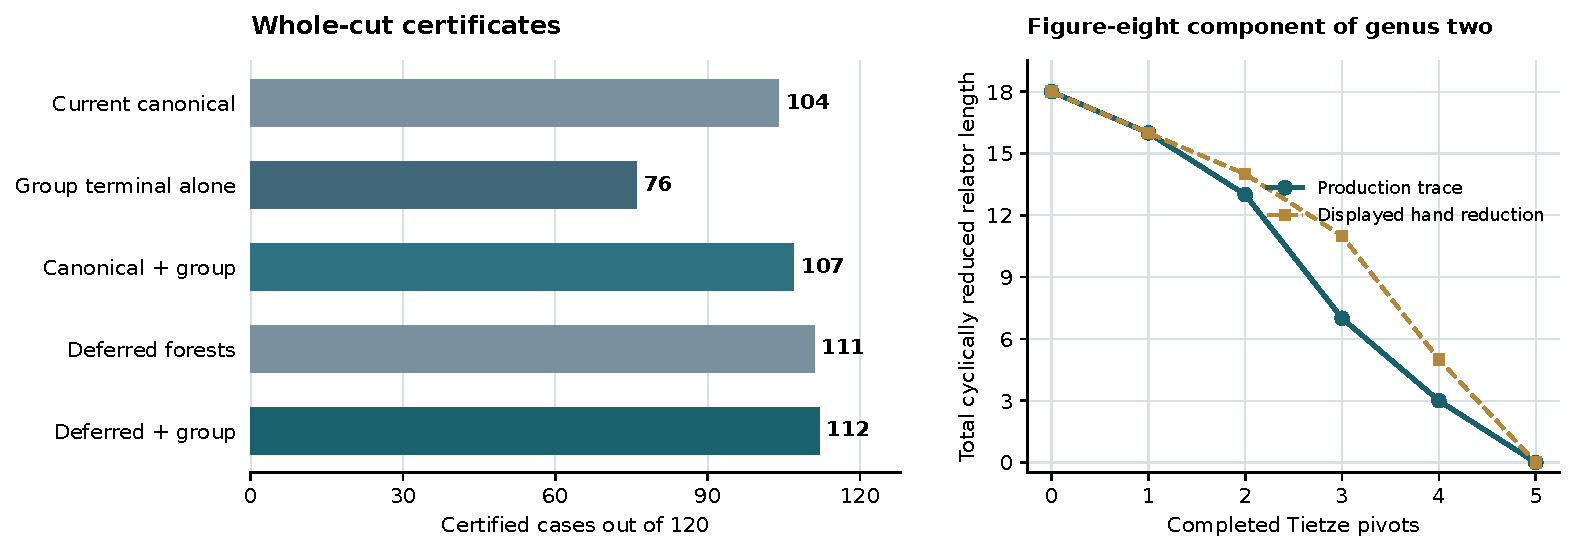
\includegraphics[width=\linewidth]{figures/coverage_and_trace.pdf}
\caption{Left: certified whole-cut coverage on the retained 120 cases.
Right: exact accepted relator lengths for the difficult figure-eight
component. Coverage and word lengths are exact counts, not timing estimates.}
\label{fig:coverage-trace}
\end{figure}

The practical integration decision is therefore conservative: preserve the
geometric fast path and expose the group terminal as an opt-in fallback.
Its main new value is additional certified coverage and a finite algebraic
terminal interface. Latency improvements depend on the surrounding scheduler
and which expensive alternatives the new certificate avoids.

% Integration notes: requires amsmath, amssymb, amsthm and theorem/proposition.
% Approximately 3--5 article pages after house-style compression if needed.

\section{From terminal certification to global complexity}
\label{sec:global-bridge}

The target considered here is
\[
 n^{O(\log n)}=\exp\bigl(O((\log n)^2)\bigr),
\]
where $n\geq2$ is the original diagram size.  The broader term
\emph{quasi-polynomial} also permits higher fixed powers of $\log n$ in
the exponential.  We distinguish these bounds explicitly.  None of the
global geometric hypotheses below has been proved for every native
hierarchy state in this package.

The new terminal algorithm removes one local obstruction: a source cut
with disk parallelity bases can be accepted through a signed group proof
even when its unsigned stopping core is large.  It does not produce the
surfaces leading to that cut, control the number of candidates, or
transport a boundary pattern through subsequent cuts.  The following
results identify precise ways to control those remaining costs.

\subsection{Amortized branching, including long repair sequences}

Consider the full finite computation tree of a hierarchy search.  A
node can be a genuine choice of cutting surface, a conjunction requiring
several cut pieces to be solved, or a deterministic repair.  Count every
recursive subproblem, including unsuccessful candidates.  Cheap rejected
candidates may instead be charged to the node's local work, provided
their entire generation and rejection cost is bounded there.

\begin{proposition}[An amortized branching bound]
\label{prop:entropy-search}
Suppose the following conditions hold for inputs of size $n$.
\begin{enumerate}
\item The search has a proved sound and complete hierarchy specification.
      Source creation, candidate generation, admissibility checking,
      marked transport and terminal discovery and verification cost at most $n^C$
      per node and per emitted recursive edge.  All required encoded
      states and local source proofs have at most $n^C$ bits.
\item Every root-to-leaf path has at most $n^C$ nodes.
\item If $b(v)\geq1$ is the number of children of a nonleaf node, then
      every root-to-leaf path $P$ satisfies
      \[
         \sum_{v\in P\text{ nonleaf}}\log_2 b(v)
                      \leq A(\log_2 n)^2.
      \]
\end{enumerate}
Then the total search, including unsuccessful candidates, costs
$n^{O(\log n)}$ bit operations.

A local sufficient condition for the third hypothesis is a certified
integer mass $1\leq M(v)\leq n^D$, nonincreasing along deterministic
edges, for which every branching edge $v\to w$ satisfies
\begin{equation}
 \log_2 b(v)\leq
 K\bigl((\log_2 M(v))^2-(\log_2 M(w))^2\bigr)+e(v,w),
 \label{eq:quadratic-log-charge}
\end{equation}
where all charges are nonnegative and their sum on each path is
$O((\log n)^2)$.
\end{proposition}
\begin{proof}
Assign equal conditional probability $1/b(v)$ to every edge leaving
each nonleaf node.  A leaf $\ell$ has probability
\[
 p_\ell=\prod_{v\in P_\ell}b(v)^{-1}\geq
             2^{-A(\log_2 n)^2}.
\]
Leaf probabilities sum to one.  Hence there are at most
$2^{A(\log_2 n)^2}$ leaves.  Every node lies on a root-to-leaf path, so
the node count is at most the maximum path length times the number of
leaves.  The edge count is smaller than the node count.  Multiplying by
the stated local bit cost proves the bound.

For the sufficient condition, sum~\eqref{eq:quadratic-log-charge} along
a path.  The squared-log terms telescope; deterministic edges have zero
branching cost and nonnegative potential drop.  The initial potential
is at most $D^2(\log_2 n)^2$, and the accumulated charges have the stated
bound.  This gives the required path sum.
\end{proof}

For example, if every branching child has mass at most half its parent
and $b(v)\leq M(v)^K$, then~\eqref{eq:quadratic-log-charge} holds with
zero extra charge.  Indeed, with $x=\log_2 M(v)\geq1$, the potential
drop is at least $x^2-(x-1)^2=2x-1\geq x$.  Thus a balanced
marked-cut theorem with polynomially many local alternatives is enough,
even if polynomially long deterministic repairs occur between its
branching steps.  The mass need not be the number of represented normal
disks; it must be a source-certified quantity with the proved decrease.

The path-length and encoding hypotheses have independent roles.  A
branching estimate does not bound an arbitrarily long unary computation,
and a bounded number of handle families does not bound the bit length of
their endpoints or the number of newly split marking intervals.  The
terminal cost is polynomial when the current $t$, profile list, integer
bit mass and source-proof size are polynomial in $n$.  This fact does
not establish the corresponding transport bounds for a successor.

\subsection{An exact small terminal key supplied by the new compiler}

The signed disk-base compiler has a useful compression property beyond
its one-shot runtime.  Here $W$ is the authenticated compact orientable
PL whole cut, every component has nonempty boundary, and every parallelity
base is a disk.  Write $a,m$ for its initial generator and relator counts
and $h_3$ for its source three-handle count.  The source ledger is
\[
 \chi(W)=c-a+m-h_3,
 \qquad r_0:=c-\chi(W)=a-m+h_3.
\]
The whole-cut criterion says exactly that $W$ is a union of handlebodies
when its component-group free product is free of rank $r_0$.

\begin{proposition}[Exact residual terminal kernel]
\label{prop:terminal-key}
Apply any independently verified finite Tietze prefix to the compiled
presentation.  Suppose $s$ surviving generators occur in no remaining
relator.  Remove these generators from the displayed presentation and
call the remaining presentation $Q$.  Put $r_*=r_0-s$.  Then
\begin{equation}
 W\text{ is a union of handlebodies}\quad\Longleftrightarrow\quad
 G(Q)\cong F_{r_*},
 \label{eq:residual-terminal}
\end{equation}
where the right side is false for $r_*<0$.

Let $k\geq1$ bound the number of generators, relators and literal letters
of $Q$ in total.  Impossible target ranks can be rejected immediately.
For $0\leq r_*\leq k$, compact relabelling gives a key $(Q,r_*)$ with
$O(k\log(k+2))$ bits, and there are
$2^{O(k\log(k+2))}$ such keys.  Normal-coordinate magnitudes and
isolated-ball multiplicities do not occur in this terminal key.
\end{proposition}
\begin{proof}
The full current group is $G(Q)*F_s$.  If $G(Q)\cong F_{r_*}$, its
free product with $F_s$ has rank $r_0$, giving the forward terminal
conclusion.  Conversely, if $G(Q)*F_s\cong F_{r_0}$, then $G(Q)$ is an
embedded finitely generated subgroup and hence free.  Abelianization
shows that its rank is exactly $r_0-s$.  This proves the equivalence.

If the required rank is negative the test is already negative.  A free
group presented on at most $k$ generators cannot have rank exceeding
$k$, so values outside $0\leq r_*\leq k$ can be separated immediately.
Encode the words with row separators over a signed alphabet of at most
$k$ generators.  The encoded string has $O(k)$ symbols from an alphabet
of $O(k)$ symbols, together with the generator count and target rank.
This proves both the bit bound and the counting bound.  The source
compiler's Euler formula shows that isolated balls cancel between $c$
and $\chi(W)$, while a verified Tietze prefix eliminates all dependence
on the original geometric labels for this algebraic predicate.
\end{proof}

This is an exact reduction of the terminal predicate, not an algorithm
for deciding arbitrary group freeness.  The present signed policy is
still one-sided.  Equal syntactic keys permit reuse of an algebraic
certificate after replaying the source compiler and the relabelling map.
Each source occurrence still needs its own authenticated binding.  A
cached greedy refusal remains a refusal of that policy.

The initial active key has $O(t\log(t+2))$ bits.  If future normalizations
guarantee residual size
\[
       k\log(k+2)=O((\log n)^2),
\]
there are at most $n^{O(\log n)}$ distinct relabelled syntactic terminal
keys.  In particular $k=O(\log n)$ gives the smaller bound
$n^{O(\log\log n)}$.  The parameter is the remaining signed
presentation size, not the old unsigned deferral number: the earlier
$q$-block geometric stopping family reduces to the empty residual even
though its raw deferral is $q$.

This cache cannot identify hierarchy states.  Equal abstract groups and
Euler data do not identify peripheral curves, marked faces, or admissible
next surfaces.  Nor does a small number of terminal keys bound the cost
of generating the geometric states that reach them.

\subsection{A precise marked-interface route to memoization}

There is a distinct route when many search histories give the same
future marked problem.  The required equivalence is stronger than
isomorphism of the terminal groups.

\begin{proposition}[Source-replayable interface quotient]
\label{prop:marked-interface-quotient}
Suppose a sound and complete marked hierarchy specification admits
keys with the following properties, where $1\leq k\leq n^C$.
\begin{enumerate}
\item A key has at most $k$ active atoms compactly labelled in
      $\{1,\ldots,k\}$, at most $O(k)$ incidence
      and cyclic-order records, and at most $O(k)$ references to a fixed
      source dictionary of at most $n^C$ exact objects.  The dictionary
      has polynomial total bit mass.  Each record has bounded arity and
      uses only atom labels, dictionary labels and a fixed finite alphabet.
\item Equal keys have source-replayable equivalences preserving the
      entire continuation problem: boundary pattern, orientations,
      peripheral data, admissibility and the correctness of all cuts.
      A representative key has at most $n^C$ candidate rules with at most
      $n^C$ child keys each, generated and checked in polynomial time.
      These rules are complete for every source realization of that key.
\item Terminal acceptance and its certificate are computed in polynomial
      time per key, or the terminal certificates are included among the
      polynomially generated candidate rules.  Merely knowing that a
      short certificate exists does not satisfy this hypothesis.
      Each terminal proof and each local source equivalence has a
      polynomial-size, polynomially checkable representation.  The
      source-lifting verifier can compose these objects as a proof DAG
      in time polynomial in $n$ per DAG node.  Source reconstruction,
      coordinate arithmetic, reindexing and marked transport are included
      in these bounds; the proof does not require exponentially expanding
      shared histories.
\end{enumerate}
Then the hierarchy can be solved in
\[
 \exp\bigl(O(k(\log n+\log(k+2)))\bigr)\operatorname{poly}(n)
\]
time.  In particular $k=O(\log n)$ yields $n^{O(\log n)}$.
\end{proposition}
\begin{proof}
There are at most
\[
 (n^C)^{O(k)}(k+1)^{O(k)}
   =\exp\bigl(O(k(\log n+\log(k+2)))\bigr)
\]
keys.  Generate the reachable quotient once, reusing every previously
seen key.  The number of rules and child references is the key count
times a polynomial in $n$.

A rule can require all its children to be accepted, while several rules
at one key represent alternative choices.  Thus acceptance is the least
fixed point of a finite monotone OR/AND rule system.  Maintain, for each
rule, the number of children not yet accepted; enqueue its parent when
that count reaches zero.  Each child reference is processed once.  Cycles
do not certify themselves: a key is accepted only after an accepting
terminal or a rule whose children were accepted earlier.  Back-pointers
therefore give an acyclic accepting proof, even if the explored quotient
contains cycles.  The completeness hypothesis identifies this fixed
point with the original finite-proof hierarchy problem.  The source
lifting hypothesis makes the resulting proof DAG valid for the original
marked input.  All generation, fixed-point and replay costs have the
stated bound.
\end{proof}

The common dictionary is a substantive requirement.  Its entries may be
very large integers, provided there are only polynomially many exact
entries and the total bit mass is polynomial.  If each of $k$ marked
coordinates instead varies freely over $B$ bits, the key bound becomes
$2^{O(k(B+\log k))}$.  With $k=\Theta(\log n)$ and
$B=\Theta((\log n)^2)$, this gives $\exp(O((\log n)^3))$, not the
target $n^{O(\log n)}$.  Proving that successor endpoints stay in a
small dictionary, or proving an equally strong exact normal form, is
part of the geometric work.

\subsection{The concrete next bridge and the exponent traps}

The most direct continuation from the implemented operator is a
\emph{marked balanced-cut theorem}: after source-authenticated
parallelity compression, either the entire piece has disk bases and a
bounded signed terminal certificate, or a polynomially generated,
complete family of marked cuts satisfies the mass charge in
\eqref{eq:quadratic-log-charge}.  Every chosen successor must retain
polynomial bit size and an exact transport of its inherited pattern.
The new finite group compiler enlarges the acceptable terminal class;
the missing theorem is the guaranteed arrival in that class or the
controlled progress of every recursive alternative.  A proof that a
particular word policy always succeeds on the guaranteed terminal class
would be required; its current Fibonacci counterexample prevents a
general freeness-completeness claim.

There are three common accounting failures.  Polynomial local work at
polynomial branching depth can still cost $2^{n^{\Omega(1)}}$ even with
two children per level.  A branching factor $n^{O(\log n)}$ at each of
$O(\log n)$ levels gives
$n^{O((\log n)^2)}=\exp(O((\log n)^3))$.  By contrast, multiplying a
total call count $n^{O(\log n)}$ by a per-call cost
$n^{O(\log n)}$ preserves $n^{O(\log n)}$: exponents add for total
work, whereas branch choices multiply along a path.  Finally, counting
only successfully emitted surfaces omits the potentially dominant cost
of unsuccessful surface searches.  Both propositions above explicitly
charge those searches and require a complete candidate mechanism.

\paragraph{Recheck of the native constants.}
The bounds $a\leq74t$ and $m,L\leq78t$ remain valid for the present
source format.  Their word-length argument uses the source validator's
exclusion of reverse-edge identifications and its circle-link condition:
an interior edge-link traversal visits each local tetrahedral edge
occurrence exactly once, so all wedge lists total at most $6t$; at most
two endpoint ranks double this to $12t$.  The additional annular words
use at most the $66t$ authenticated ports once in total.  These bounds
do not constrain the full base-profile list, integer bit mass, source
proof length, transported marking intervals, or the tetrahedron count
of later successor states.  Those quantities cannot be absorbed into
the constants $74$ and $78$.

\section{Further research questions and proposed work programme}
\label{sec:research}

The next phase should be driven by precise missing lemmas and adversarial
families. A successful experiment is useful when it identifies a parameter or
falsifies an attractive universal claim. The figure-eight improvement and the
Fibonacci-word refusal together give a concrete starting point: signed
substitution matters, but singleton access is not a complete basis-change
mechanism. The following questions are ordered roughly from immediate native
work to the global geometric bottlenecks.

\subsection{Immediate terminal and implementation questions}

\begin{question}[Recover the two admitted disk-base stalls]
Can explicit source-aware Nielsen transformations expose defining generators
in the two remaining disk-base word stalls, while keeping a polynomial total
word-size budget? First retain their full signed presentations and compare
different generator bases. Require exact automorphism certificates and replay
of the original words. Success means new whole-cut certificates or a small,
repeatable obstruction to the proposed basis policy; a change in abelianized
rank alone does not count.
\end{question}

\begin{question}[A stronger bounded algebraic policy]
What is the smallest additional move family that resolves automorphic
images such as $\langle a,b\mid\varphi^k(a),\varphi^k(b)\rangle$ efficiently
without making discovery exponential in the rank? Candidate moves include
certified Nielsen basis changes, relator multiplication and controlled
temporary length growth. Charge both number of moves and intermediate literal
or compressed bit size. A short certificate found by unbounded search is a
different achievement from a bounded discovery algorithm.
\end{question}

\begin{question}[Package the early homology obstruction]
Can the partial-trace condition $z>h_3$ be exported as a compact independent
whole-cut obstruction certificate? The theorem already proves its soundness.
The implementation task is to retain the verified prefix, authenticate the
source count and expose a clearly typed result. Such a result can prune a
terminal candidate while preserving the possibility that a different normal
surface gives a useful hierarchy.
\end{question}

\begin{question}[Reuse authenticated source work across the portfolio]
Can the geometric and group terminals share one immutable source/boundary
packet and one explicit work ledger? The present opt-in wrapper repeats source
preparation after a refusal. A useful refactor would reduce measured failed-path
latency and eliminate the two-stage orbit allowance, while preserving legacy
certificate output and callback semantics. Measure complete successful queries
and inconclusive queries separately, including packet serialization.
\end{question}

\begin{question}[Incremental relator substitution]
Can inverted occurrence lists, lazy substitutions or straight-line programs
reduce the current $O(N^4)$ discovery bound and its constants without changing
the selected minimum-length move? An occurrence index can avoid scanning words
that do not contain the pivot, but exact cyclic cancellation and candidate
comparison still need a proof. Record total changed-word work, transient word
length and certificate replay cost, rather than only counting chosen pivots.
\end{question}

\subsection{Larger source classes and geometric certificates}

\begin{question}[Extend the compiler beyond disk bases]
For a compact base surface with boundary, its group is free but its boundary
curves have specified words. Can a graph-of-spaces compiler retain these words,
cyclic edge groups for full annuli, and trivial edge groups for intervals with
an active size controlled by ports and encoded base complexity? A boundary loop
of a positive-genus one-boundary surface is not a free generator. Replacing it
by one would be unsound. Very large encoded genus may also force a long
commutator word unless a justified compressed representation is used.
\end{question}

\begin{question}[Terminal residual kernels in real hierarchies]
After geometric peeling and signed simplification, is the terminal residual
size logarithmic in the original diagram size on a geometrically defined
class? The exact semantic kernel in the preceding section makes this a
well-posed parameter question. The old linear-deferral ball family no longer
obstructs it, since signed elimination solves every block. The Fibonacci basis
family shows that raw singleton residual size is sensitive to coordinates.
A useful theorem must therefore specify allowed source-certified basis changes.
\end{question}

\begin{question}[Recover source-coordinate meridians]
When the Euler/free-group terminal certifies $H_g$, can a separate procedure
construct a complete meridian system with bounded compressed descriptions and
verified boundary carriers? The current proof uses the Loop Theorem and
Poincar\'e only for existence. Converting an abstract group basis into disks is
an additional geometric problem. A first milestone is the explicit
figure-eight genus-two component, with independently checked embedded disks
and transports to the original source charts.
\end{question}

\begin{question}[Essential boundary patterns at an algebraic terminal]
Can a bounded marked pattern be checked for the properties needed by a
hierarchy once the ambient piece is certified to be a handlebody? Merely
knowing the genus or the abstract group leaves the pattern's embedding unknown.
The desired packet should retain cyclic order, side information, slopes where
relevant, and witnesses that rule out violating disks. This is a natural point
to connect finite boundary graphs with source-coordinate meridian certificates.
\end{question}

\begin{question}[Turn apparent basis obstructions into geometric families]
Can the algebraically incomplete Fibonacci-word examples be realized and
exported by the native normal-cut constructor with controlled triangulation
size? Conversely, do the native disk-annulus sources satisfy an extra
restriction that rules out some arbitrary finite-presentation obstructions?
Producing actual face pairings and normal coordinates, rather than a plausible
attaching-word diagram, is the required experiment.
\end{question}

\subsection{The global quasi-polynomial bottlenecks}

\begin{question}[Find an amortized geometric branch potential]
Can a compressed hierarchy admit a nonnegative potential whose decrease pays
for $\log b$ at a node with $b$ genuine successor alternatives? Polynomially
many deterministic repairs are harmless if they do not replenish this
potential. Candidate ingredients include boundary pattern complexity,
nonproduct core size, a hierarchy surface's essential topology and the residual
group kernel. The local inequality in the branch-budget theorem is a concrete
target; mere lexicographic termination does not imply it.
\end{question}

\begin{question}[Construct a small marked interface quotient]
Is there a source-liftable signature on $O(\log n)$ marked interface records
that preserves every relevant continuation and terminal condition? The
signature must account for mapping-class information that group rank,
component incidence and Euler characteristic forget. For every proposed
signature, actively search for two equal-key inputs with different outcomes
under the same allowed continuation. A collision of this kind is more
informative than a high cache-hit rate on easy inputs.
\end{question}

\begin{question}[Bound candidate surfaces, not just one chosen surface]
Can the algorithm generate a complete family of geometrically useful normal
cuts in polynomial or quasi-polynomial total work at each essential branching
stage? Efficiently finding one nonseparating surface does not show it is enough
for every later repair. The statement should specify which alternatives cover
all successful hierarchies and charge the cost of rejected candidates,
coordinate generation and source validation. A short existential hierarchy
certificate is not a deterministic search bound.
\end{question}

\begin{question}[Control marking growth under repeated cuts]
Can every successor be represented in size polynomial in the original diagram
length, including all coordinates, interval endpoints, boundary patterns and
transport proofs? A core with $O(n)$ handles can still carry enormous boundary
word data. The bound must cover the complete state and certificate, not only
the geometric core or the new active group presentation.
\end{question}

\begin{question}[Connect terminal improvements to a diagram-level schedule]
Which expensive current recognizer branches can be avoided when a supplied cut
receives the new certificate? Implement a bounded experimental schedule that
records diagram-to-exterior provenance, candidate-surface cost, source cuts,
all retries and final independent verification. Report added successful knot
verdicts and total latency, preserving timeout and inconclusive semantics. The
current three added cut successes alone do not predict that outcome.
\end{question}

\begin{question}[Formalize the smallest trusted mathematical interface]
Can the disk-base graph-of-spaces compiler, signed Tietze trace and Euler count
ledger be formalized separately from a full normal-surface library? The finite
combinatorial layer is a promising first target. The topological theorem could
initially be stated with explicit classical assumptions, then connected to a
formal 3-manifold development. This would expose exactly which source geometry
invariants must be certified rather than inferred from implementation history.
\end{question}

\subsection{Suggested milestones}

The first milestone is a reviewed integration of the present opt-in terminal,
with the three added native cases and five Euler-obstruction packets kept as
permanent regressions. Next, extend the residual algebraic policy and measure
its effect on actual source presentations; do not optimize arbitrary group
examples without confirming that they model the geometric bottleneck. In
parallel, construct source-coordinate marked meridian data for the figure-eight
target and evaluate the nondisk graph-of-spaces compiler.

The decisive theoretical milestone is then either a logarithmic amortized
branch budget or a complete small marked-state quotient, with polynomial state
size and proof lifting. The new terminal makes one local operation finite and
cheap in the relevant encoding. It also supplies exact refusal information.
Those are useful components of a complexity proof, while the global geometric
claims above remain the substantive research problem.

\appendix
\section{Package contents, reproduction and integration}
\label{sec:reproduction}

\subsection{Files and dependencies}

The archive is intended to be placed in \code{docs/incoming} or assigned a new
research-report number after review. Its root contains a README, integration
instructions, a claim ledger, source provenance, license notes and SHA-256
checksums. The article directory contains this complete \LaTeX{} source,
section files, bibliography, reproducible vector figure and compiled PDF.
The integration directory contains a unified patch and a complete eleven-file
overlay under repository-relative paths.

The production extension uses only the Python standard library. The delivered
audit scripts additionally use Regina 7.4 for explicit independent comparisons;
the saved run used Python 3.12.14. Regenerating the scientific figure requires
Matplotlib. Building the article uses pdf\LaTeX{} and BibTeX, with ordinary
mathematical and typography packages. Versions and exact source hashes appear
in the result files. The package does not vendor the whole ProveIt runtime or
third-party software.

\begin{longtable}{P{0.39\linewidth}P{0.54\linewidth}}
\toprule
Path & Purpose \\
\midrule
\endhead
\path{article/Euler_Group_Terminals.tex} & Main article and full proofs \\
\path{article/Euler_Group_Terminals.pdf} & Rendered article \\
\path{integration/euler_group_terminals.patch} & Patch against the pinned production source \\
\path{integration/overlay/} & Six new production modules, three new test modules and two updated entry-point modules \\
\path{fixtures/} & Exact 106 historical and 14 interior-extension sources \\
\path{certificates/group/} & All 76 complete new group-terminal packets \\
\path{certificates/figure_eight.json} & Convenient standalone target packet, also used by the independent algebraic audit \\
\path{certificates/euler_defects.json} & Five source-bound free-group proofs with exact positive $b_2$ \\
\path{comparison/deferred/} & Four unchanged attributed incoming modules used only for the deferred comparison \\
\path{results/} & Coverage audit, group audit, regression logs, replay reports, raw benchmark samples and methodology \\
\path{tools/} & Portable replay, audit, benchmark and figure-generation commands \\
\bottomrule
\end{longtable}

\subsection{Replay before rediscovery}

Apply the patch to a separate checkout at the pinned commit as described in
\code{INTEGRATION.md}. From the unpacked package, set a task-specific shell
variable to that checkout's fast runtime:
\begin{lstlisting}[language=bash]
fast_root=/path/to/ProveIt/Topology/UnknotRecognition/fast
python tools/verify_packets.py --fast-root "$fast_root"
python tools/audit_euler_defects.py --fast-root "$fast_root" \
  --replay-only certificates/euler_defects.json \\
  --output /tmp/euler_defect_replay.json
\end{lstlisting}
The first command uses the existing public whole-cut verifier dispatch, so it
checks the new schema through the intended integration interface. It requires
no Regina installation and performs no proof discovery. Malformed JSON is
rejected before replay, including duplicate keys and floating-point values.
The source packets use the established exact integer codec for huge values.

Reproduce the independent algebraic audit with:
\begin{lstlisting}[language=bash]
python tools/audit_freeness.py --fast-root "$fast_root" \
  --target certificates/figure_eight.json \
  --output /tmp/independent_freeness.json
\end{lstlisting}
This command requires Regina and must run without Python's \code{-O}, since
the research audit uses assertions. It produces the 10203-presentation corpus,
source hashes, exact checks and counterexamples. Omitting the target omits its
two components and leaves 10201 presentations.

The complete fresh native audit is:
\begin{lstlisting}[language=bash]
python tools/audit_native.py --fast-root "$fast_root" \
  --output /tmp/native_audit.json --packets /tmp/group_packets
\end{lstlisting}
It creates an isolated runtime for the deferred comparison, uses the four
preserved modules and replays those positives as well. It launches literal
Regina oracle calls with the documented 4096-disk cap and per-case timeout.
The command does not modify the production checkout. Its \code{--resume}
option requires matching source identities; the main report explains the
single integer-transport recovery in the saved run.

\subsection{Tests and measurements}

In the integrated fast runtime, run:
\begin{lstlisting}[language=bash]
python -m unittest tests.test_free_group_elimination \
  tests.test_euler_group_terminal tests.test_source_cut_group -v
python -m unittest discover -s tests -v
\end{lstlisting}
The saved focused and full runs contain 33 and 1749 passing tests,
respectively. Existing fixture directories from the repository are needed for
the full suite; the eleven-file overlay alone is not a standalone copy of all
ProveIt dependencies.

For descriptive complete-query timings, run after other benchmark and audit
jobs have finished:
\begin{lstlisting}[language=bash]
python tools/benchmark_terminals.py --fast-root "$fast_root" \
  --output /tmp/terminal_benchmarks.json
\end{lstlisting}
The script preserves unsuccessful statuses and case timeouts. It never forms
a recognition speed ratio using an inconclusive arm. The one-tetrahedron
families exercise binary multiplicity; the new target cases exercise changed
terminal coverage. The raw A/A arms help identify timing noise. Neither these
few samples nor a log-log chart establishes an asymptotic exponent.

\subsection{Build and inspect the article}

From the package root:
\begin{lstlisting}[language=bash]
python tools/generate_figures.py
bash article/build.sh
\end{lstlisting}
The build script changes into its own article directory and runs pdf\LaTeX,
BibTeX and two final pdf\LaTeX{} passes. The source bibliography uses primary
literature and pinned repository links. The supplied PDF was compiled, rendered
to page images and visually checked; the final build log is retained. There
are no external image downloads or generated raster illustrations required to
rebuild the article.

\subsection{Merging with the incoming deferred work}

The patch is verified against the exact current production baseline. The
incoming deferred overlay and this patch both edit
\code{normal\_cut\_handlebodies.py}; applying one full-file overlay on top of the
other would discard logic. Integrate their argument handling and fast-path
choice deliberately. Preserve the new public verifier dispatch and the old
certificate schemas, then rerun the focused checks, the new target and the
combined corpus. The 112-case union is evidence for this combined portfolio's
potential coverage; the package does not claim that the incoming
\code{forest\_strategy} option is already merged into the new wrapper.

\section{Additional logical boundaries}

\paragraph{Closed components.}
The nonempty-boundary condition in Theorem~\ref{thm:free-euler} is essential.
The closed manifold $S^1\times S^2$ has $c=r=1$ and $\chi=0$, so it satisfies
$\chi=c-r$ while not being a handlebody. The current source validator excludes
this input. Reusing the theorem in a broader source API requires establishing
the boundary condition for every cut component or adding a separate closed
component classification.

\paragraph{Source authentication before rank arithmetic.}
The same numerical presentation, genus and Euler arrays can be attached to
unrelated geometry. All numerical equations in the terminal gate are
conditional on the verified presentation actually presenting the whole-cut
groups. Neither a checksum nor a plausible genus histogram supplies that
topological identification. Signs at loop one-handles, full annular disk
attachments, interval bridges, core two-handles and binary isolated balls are
all part of the binding.

\paragraph{Certificates versus constructive homeomorphisms.}
The trace certifies a group isomorphism and the theorem determines the
unmarked three-manifold type. It does not produce an explicit PL homeomorphism
to a standard handlebody. A downstream algorithm requiring meridian disks,
boundary embeddings or a re-triangulated marked successor must request and
verify those objects separately.

\paragraph{Historical scope.}
The compression data model, raw stopping-set analysis and deferred-forest
results are attributed to the preceding ProveIt work. The topological ingredients
are classical. The contributions claimed here are the particular complete
source-bound disk compiler and its active bounds, the Euler-checked signed
terminal and exact relator ledger, the residual terminal reduction, the new
native certificates, and the explicit conditional research programme. No claim
of exhaustive historical priority or a completed quasi-polynomial recognition
theorem is made.

\section{A profile-directed bounded-expansion certificate}
\label{sec:bounded-expansion}

The mixed Pachner profile identifies substantial compressed-orbit overhead on
small represented universes. Expansion can be a sensible small-case method
only if the decision to expand is itself tied to encoded input size. This
design lemma gives an explicit safe guard and a complete exact witness. It
uses standard graph connectivity, and is proposed as a future source-query
adapter rather than an implemented normal-cut backend.

\begin{proposition}[Polynomially guarded explicit orbit replay]
\label{prop:guarded-expansion}
Let $q$ interval pairings generate an equivalence relation on
$\{0,\ldots,U-1\}$. Each pairing is an affine bijection of integer intervals
with slope $+1$ or $-1$, specified by binary endpoints. Let $N\geq2$ be the
total bit length of the complete query, including any binary piecewise-constant
additive weights in explicitly listed finite-dimensional integer vectors
(or sparse vectors over explicitly named coordinates). Fix a constant $d\geq1$.

When $U\leq N^d$, the exact orbit partition admits a certificate consisting of
at most $\max\{U-1,0\}$ source-witnessed forest edges, using
$O(U(\log(U+1)+\log(q+1)))$ bits. Discovery and independent replay, including
the total weight of every orbit, have polynomial bit complexity in $N$ for
certificates within this size bound. If a separate compressed backend costs
$T_{\mathrm{comp}}(N)$, this guarded hybrid has bound
$T_{\mathrm{comp}}(N)+\operatorname{poly}_d(N)$; in particular it preserves a
polynomial or quasi-polynomial complexity class.
\end{proposition}
\begin{proof}
Create one graph vertex per point and, for every source pairing and every point
in its domain, the corresponding undirected relation edge. There are at most
$qU$ such edges. A spanning forest can be constructed by a standard
union-by-size disjoint-set traversal. Record each accepted forest edge by its
source pairing index and domain point; the other endpoint is reconstructed
from that pairing. Distinct source indices and points require the stated bit
length. The forest has $U-c$ edges, where $c\geq1$ is its component count when
$U>0$; the empty universe has the empty certificate.

For independent replay, check the domain and affine image of every listed
edge, reject loops or repeated-cycle edges in the claimed forest, and compute
its components by a separate graph traversal. Then enumerate every source
pairing edge and check that its endpoints lie in one forest component. Every
forest edge belongs to the source relation, so forest connectivity is contained
in the generated equivalence relation. The last check proves the reverse
containment. Thus the partition is exact: neither splitting a true orbit nor
merging distinct orbits can pass.

Evaluate the source weight description at each point and add the resulting
integer vectors over its certified component. A direct scan of the input
weight records at each point already has polynomial cost when $U\leq N^d$.
With $R$ input weight records and largest coefficient bit length $b$, each
resulting coordinate sum has $O(b+\log(R+1)+\log(U+1))$ bits, and the number of
explicitly named weight coordinates is at most $N$. All graph work, enumeration and exact
arithmetic are consequently polynomial in $N$ for fixed $d$. The guard is
tested on binary integers before allocating any point array. For larger $U$,
the explicit algorithm is not entered at all.
\end{proof}

The proposal still needs a native schema and source adapter for each weighted
query and each auxiliary fibre-cover query. The source must authenticate the
pairings and weight descriptions just as it does for compressed orbit traces.
An explicit witness for a small universe is not permission to expand a huge
normal surface. The exponent $d$ is fixed independently of numerical weights;
the threshold depends on their encoded bit lengths. Benchmarking both modes on complete source-bound
queries would determine a practical threshold. This is a concrete next
performance experiment supported by the observed profile and by a proved
encoded-complexity guard.

\bibliographystyle{plain}
\bibliography{references}
\end{document}
